\documentclass[12pt, titlepage]{article}
\usepackage[normalem]{ulem}
\usepackage{color}
\usepackage{enumitem}
\usepackage{booktabs}
\usepackage{tabularx}
\usepackage{float}
\usepackage{indentfirst}
\usepackage{graphicx}
\graphicspath{{img/}}
\usepackage{hyperref}
\hypersetup{
    colorlinks,
    citecolor=black,
    filecolor=black,
    linkcolor=black,
    urlcolor=blue
}
\usepackage[round]{natbib}

\title{SE 3XA3: Design Documentation \\ Module Guide}

\author{Team 3 - Hextron
		\\ Jason Li lij107
		\\ Scott Williams willis12
		\\ Yousaf Shaheen shaheeny
}

\date{December 6, 2017}



\begin{document}

\maketitle

\pagenumbering{roman}
\tableofcontents
\listoftables
\listoffigures
\newpage

\begin{table}[]
\caption{\bf Revision History}
\begin{tabularx}{\textwidth}{p{3cm}p{2cm}X}
\toprule {\bf Date} & {\bf Version} & {\bf Notes}\\
\midrule
November 10, 2017 & 1.0 & Revision 0 \\ \hline
December 6, 2017 & 1.1 & \begin{itemize}[leftmargin=0cm,itemindent=.5cm,labelwidth=\itemindent,labelsep=0cm,align=left,itemsep = 0mm,nosep]


  \item Overhaul of anticipated and unlikely changes.
  \item Overhaul and additions to module list.
  \item Added module hierarchy diagram.
  \item Recategorised the modules.
  \item updated both traceability matrices.
  
\end{itemize} \\
\bottomrule
\end{tabularx}
\end{table}
\vspace*{\fill}


\newpage
\pagenumbering{arabic}
\newpage
\section{Introduction}
This is the module guide for the remake Hextris, an altered version of a open sourced online game that adds elements of tetris to a hexagon based reaction game. This guide is for the explanation of the design as well as the breakdown of the various modules used in the creation of the game. The document is also used to improve updates and fixes breaking down the game into more manageable chunks for future developers and designers to use. It also lends itself to allow for an easier time for  validating the requirements set by the SRS in decomposing the projects. The module guide complements the MIS document in providing a better explanation of the separate functions and classes provided by the MIS. 

\subsection{Overview}
The document will begin with the changes as well as the confirmed differences to our project highlighting the new differences and what was kept the same. The document will then list and explain the decomposition of the various modules. The document will then go over the module hierarchy, finishing with a traceability matrix.



\section{Anticipated and Unlikely Changes}
The following section outlines the changes that were made to the project. Some of these changes are ones we anticipated and some are unlikely changes.

\subsection{Anticipated Changes}
As the project goes on, the team discover certain aspects of the project that need to be changed in the future. These anticipated changes are all changes that are to be executed by modifying a single module for each change. The following is a list of anticipated changes the team has determined to be necessary for the completion of the project.

\begin{enumerate}[label=\textbf{AC\arabic*:}]
{\color{blue}
  \item Modify the game to make it mote difficult, crate obstacles for the player.
  \item Addition of new features to the game to differentiate it from the original.
  \item Decrease complexity of some features to be added.
  
}
  
  
  
  
  \item \sout{Decreasing the amount of block variations to be added to the final product.}
  \item \sout{Development a block destruction algorithm.}
  \item \sout{Decrease the scope of some of the features to be added for the user interface.}
  \item \sout{Added implementation of a fill algorithm for usage when matching blocks are to be found.}
  \item \sout{Added implementation of a fill algorithm for usage when matching blocks are to be found.}
\end{enumerate}

\subsection{Unlikely Changes}
\sout{During the implementation and production of the product, certain things problems arise that facilitate the need for a modification to a certain module. These problems can be resolved through modifications to the modules respective to each problem. These problems cause the need for changes that were not expected to be made by the team prior to the implementation.}\\

{\color{blue}During the specification phase of the project, certain specifications arise that are unlikely to change. These specifications are things that are fundamentally important to the project and should not be changed to ensure the quality of the final project. The following is a list of some design decisions made during the specifications that are unlikely to change during the course of the project.}
 


\begin{enumerate}[label=\textbf{UC\arabic*:}]
{\color{blue}%begin coloring
  \item The player controls will not be changed as the current scheme is more than suitable.
  \item The game rules will also not be changed to ensure that the final product resembles Hextris.
  \item The different colors of trapezoids will remain at four.
  \item The speed at which the trapezoids fall onto the hexagon and the rate at which it increases will remain unchanged.
  \item The game over condition will not be changed and will remain at a height of 8 trapezoids.
  
}%end coloring 
  \item \sout{Certain animation to the hexagon object will be omitted.}
  \item \sout{Physics of the trapezoids will need to be modified to restrict unwanted movement.}
  \item \sout{Player controls and menu interface remains unchanged.}
  \item \sout{Added background music for a more appealing interface when the game is being played.}
  \item \sout{The pause button was changed from 'P' to the Space Bar.}
\end{enumerate}

\section{Module Hierarchy}
The following section is an overview of the modules to be implemented in the final product. The modules are categorized into three categories; Hardware-Hiding Modules, Behaviour-Hiding Modules, and Software Decision Modules. The following is a table detailing the decomposition of the modules into their respective categories.

\begin{enumerate}[label=\textbf{M\arabic*:}]
  \item HexagonBehaviour(Player Controller) - This module dictates the movement and modification of the hexagon game object within the game.
  \item LevelManager - This module manages the boot processes of the game.
  \item MusicPlayer - This module finds and plays the music file while the game is being played.
  \item PauseManager - This module implements the pause functionality of the game.
  \item Spawner - This module generates a trapezoid of a random colour and a random location of the six defined locations to be dropped in the game.


  \item \sout{TrapezoidBehaviour - This module handles the main physics of the trapezoids that are to be dropped onto the hexagon object. This includes the motion, scaling, collision, and position of the trapezoids. This module includes two scripts; TrapezoidTransform and TrapezoidCollision.}
  
  
  \item Game Interface - This module handles the drawing of the various game objects as well as the various screens. Additionally it handles the frame to frame updates keeping track of time and score. Mostly of the Game interface is embedded and linked with the unity engine.
  
  
{\color{blue}
  \item TrapezoidTransform - This module scales the trapezoids so that they are the correct size as they approach the center hexagon. 
  
  \item TrapezoidCollision - This module handles the main physics and collisions of the trapezoids with each other and the black center hexagon. It also contains the floodfill algorithm that deals with the block elimination. It also stores the position of each trapezoid in a grid.

  \item EffectScript - This module handles the trapezoid elimination sound effect.
  
  \item LocalLeaderboard - This module deals with the updating of the local leaderbaord for when a new highscore is obtained.
  
  \item RandomTips - This module gives the user helpful tips and hints for when they encounter a game over screen.
}
\end{enumerate}

\begin{center}
\begin{table}[h!]
\centering
\begin{tabular}{ |c| c| }\hline

 \textbf{Level 1}         & \textbf{Level 2}  \\ \hline
 
 
 Hardware-Hiding Module   & \\ \hline
 
 
 Behaviour-Hiding Module  & \begin{tabular}[c]{@{}l@{}} M1\\M4\\M5\\M8\\M9\\M11\\M12\end{tabular}            \\ \hline
 
 
 Software Decision Module & \begin{tabular}[c]{@{}l@{}} M2\\M3\\M7\\M10\end{tabular}            \\ \hline
\end{tabular}
\caption{Module Hierarchy}
\end{table}
\end{center}

\section{Connection Between Requirements and Design}
Certain design decisions needed to be made in order to facilitate the requirements outlined in the SRS documentation. For the random trapezoid generation functionality, the team decided to choose between one of four colours and one of six positions for each face of the hexagon. The movement function requirement of the trapezoids was facilitated through setting a velocity vector for each trapezoid pointing to the center of the hexagon. The speed of the falling trapezoids increasing was designed by increasing the magnitude of the velocity vector by a scaling factor that is directly related to the total time the current game is running. The game will support up to eight trapezoids stacked up on each face of the hexagon. A limit was set on the hexagon and is to be checked each time a new block is dropped. If the height of the stack exceeds eight trapezoids, then the game would end. The rotation of the hexagon was is to be controlled by the user. The decision made was that the rotation is to be controlled by the left and right arrow keys on the keyboard. The left arrow key rotates the hexagon by 60 degrees to the left and the right arrow key rotates the hexagon by 60 degrees to the right. For the pause functionality of the game, the team decided to set the time scale value in the code to 0 to simulate the freezing of time in the game. The above requirements and their corresponding design decisions were made by the team to ensure the quality and the completion of the project.

\section{Module Decomposition}
The following section outlines each module defined above in more detail. The section talks about the secrets and services of each module. It also outlines what the module was implemented by. The section discusses certain aspects of each module that pertains to the functionality of the module in question.

\subsection{Hardware Hiding Modules}
\noindent This section outlines the modules categorized in the Hardware Hiding category. {\color{blue}However, for a project such as this one, there are no hardware hiding modules.}


\subsubsection{LevelManager (M2)}
\sout{\noindent \textbf{Secret:} Secret: Loads assets and all files from game src folder.\\
\textbf{Services:} Boots environment and assests loading the start menu activating all the other scripts to be used when the game is started.}

\subsubsection{Interface (M7)}
\sout{\noindent \textbf{Secret:} Tracks time for trapezoid generation. \\
\textbf{Services:} Handles the frame to frame updates keeping track of time and score. Mostly of the Game interface is embedded and linked with the unity engine.
}


\subsection{Behaviour Hiding Modules}
\noindent This section outlines the modules categorized in the Behaviour Hiding category.
\subsubsection{HexagonBehaviour(Player Controller) (M1)}
\noindent \textbf{Secret:} script that waits for player input to rotate the hexagon by 60 degrees.\\
\textbf{Services:} Waits for user input to dictate the movement of the hexagon for the player and then rotates the parent hexagon and all of its connected child trapezoids by the 60 degrees as well.

\subsubsection{PauseManager (M4)}
\noindent \textbf{Secrets:} Halts the other operating scripts of the game.\\
\textbf{Services:} Brings up pause menu and stop other game scripts from continuing 

\subsubsection{Spawner (M5)}
\noindent \textbf{Secret:} Creates trapezoids at random with randomized pre-set color. \\
\textbf{Services:} Creates the blocks for the player to match with fully randomized parameters for color and spawn location. Continues to create trapezoids and increases speed incrementally to increase difficulty. 

\subsubsection{TrapezoidBehaviour (M6)}
\sout{\noindent \textbf{Secret:} Applies gravity effects on spawned trapezoids and moves them towards the hexagon. \\
\textbf{Services:} Handles all aspects of the trapezoid blocks in regards to its characteristics. This includes the motion, scaling, collision, and position of the trapezoids. This module includes two scripts; Trapezoid Transform and Trapezoid Collision.}

{\color{blue}

\subsubsection{TrapezoidTransform (M8)}
\noindent \textbf{Secret:} Modifies the visual aspects of the trapezoids. \\
\textbf{Services:} This module decreases the size of the trapezoid as it gets closer to the center black hexagon. As it gets closer to the hexagon, the module decreases the size of the trapezoid.

\subsubsection{TrapezoidCollision (M9)}
\noindent \textbf{Secret:} Deals with trapezoid physics. \\
\textbf{Services:} This module deals with the main physical functions of the trapezoids. It computes collisions. It also contains the floodfill algorithm used for block elimination.

\subsubsection{LocalLeaderboard (M11)}
\noindent \textbf{Secret:}  Deals with the leaderboard.\\
\textbf{Services:} This module basically keeps the leaderboard up to date with the highest scores on the local machine.

\subsubsection{RandomTips (M12)}
\noindent \textbf{Secret:}  Provides helpful tips/hints.\\
\textbf{Services:} This module provides the user with helpful tips/hints in the case of a game over condition.

}


\subsection{Software Decision Modules}
\noindent This section outlines the modules categorized in the Software Decision category.
\subsubsection{MusicPlayer (M3)}
\noindent \textbf{Secret:} Loads background music file.\\
\textbf{Services:} Loads and plays mp3 background music file and keeps it playing. 

{\color{blue}
\subsubsection{MusicPlayer (M2)}
\noindent \textbf{Secret:} Loads assets and all files from game src folder.\\
\textbf{Services:} Boots environment and assests loading the start menu activating all the other scripts to be used when the game is started.

\subsubsection{Game Interface (M7)}
\noindent \textbf{Secret:} Load basic game GUI.\\
\textbf{Services:} Launches and initialises all game aspects and scenes needed for the game to function as intended.

\subsubsection{EffectScript (M10)}
\noindent \textbf{Secret:} Provides block elimination sound effects.\\
\textbf{Services:} This module plays a sound effect whenever a block elimination occurs.

}


\section{Traceability Matrix}
\noindent The following section outlines two traceability matrices. One outlining the Trace Between Requirements and Modules and the other outlining the Trace Between Anticipated Changes and Modules.

\begin{center}
\begin{table}[H]
\centering
\begin{tabular}{ |c| c| }\hline

 \textbf{Requirements}         & \textbf{Modules}  \\ \hline
 F1   & M5, M7, M8, M9  \\ \hline
 F2   & M2, M6, M8, M9  \\ \hline
 F3   & M2, M5, M7, M8, M9  \\ \hline
 F4   & M1, M8, M9  \\ \hline
 F5   & M1, M7  \\ \hline
 F6   & M4, M2  \\ \hline
 F7   & M5, M7, M8, M9, M10  \\ \hline
 F8   & M5, M7, M8, M9, M10  \\ \hline
 F9   & M12  \\ \hline
 F10  & M3, M10  \\ \hline
 F11  & M11  \\ \hline
 F12  & M1, M8, M9  \\ \hline
\end{tabular}
\caption{Trace Between Requirements and Modules}
\end{table}
\end{center}

\begin{center}
\begin{table}[H]
\centering
\begin{tabular}{ |c| c| }\hline

 \textbf{Modules}    & \textbf{Anticipated and Unlikely Changes}  \\ \hline
 M1   & AC2, UC1, UC5   \\ \hline
 M2   & AC3, UC5  \\ \hline
 M3   & AC2  \\ \hline
 M4   & AC3, UC1  \\ \hline
 M5   & AC1, AC2, AC3, UC2, UC3, UC4, UC5  \\ \hline
 M7   & AC2, UC1, UC5  \\ \hline
 M8   & AC1, AC2, UC3, UC4, UC5  \\ \hline
 M9   & AC1, AC2, UC3, UC4, UC5  \\ \hline
 M10  & AC2, AC3  \\ \hline
 M11  & AC2, UC2, UC5  \\ \hline
 M12  & AC1, AC2, AC3, UC5  \\ \hline
 
\end{tabular}
\caption{Trace Between Anticipated Changes and Modules}
\end{table}
\end{center}




\section{Use Hierarchy Between Modules}
Use Hierarchy between Modules: This section explains some of the interaction between the various modules. Starting with the level manager which is responsible for the startup assets of the game and the instantiation of most of the other modules. The Hexagon behaviour, Trapezoid behaviour, Game interface and Music player is then used. The spawner is non dependent on most of the other modules, continuously creating blocks until the game is paused or the game is stopped. Trapezoids generated are taken by the trapezoid behaviour which then scales and applies gravity to the blocks. Colliding with the player, the player control dictates the movement of the center hexagon. All the modules operate under the game interface which is unity's platform for frame updates and time tracking. Music player is also an independent module that provides the background music regardless the processes of the other modules.



\begin{figure}[h!]
\centering
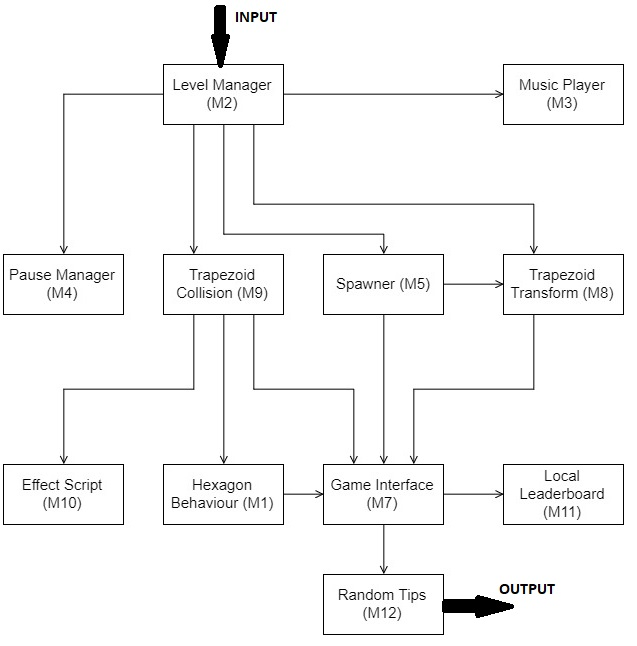
\includegraphics[width = 11cm]{ModuleHierarchyDiag}
\caption{Module Hierarchy Diagram}
\end{figure}

\newpage
\section{Schedule}
\noindent The following is the Gantt Chart schedule of the project.
\begin{figure}[H]
\centering
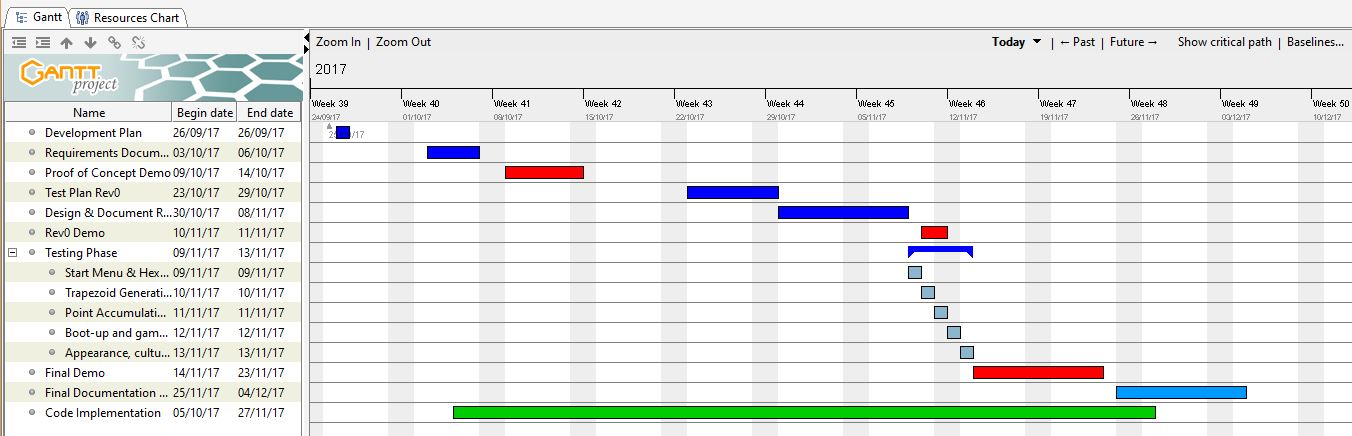
\includegraphics[width = 14cm, height = 6cm]{GanttChart}
\caption{Gantt Chart}
\end{figure}






















\end{document}